\documentclass[12pt]{extarticle}
\usepackage[utf8]{inputenc}
\usepackage[main=spanish, english]{babel}
\usepackage{csquotes}
\usepackage{graphicx}
\usepackage{fancyhdr}
\usepackage{geometry}
\usepackage{lipsum}
\usepackage{tocloft} 
\usepackage{amsmath}
\numberwithin{equation}{section}
\setlength{\jot}{14pt}
\usepackage{amssymb}
\usepackage{float}
\usepackage{caption}
\usepackage{pifont}
\usepackage[table,xcdraw]{xcolor}
\usepackage{algpseudocode}
\usepackage{algorithm}
\usepackage{booktabs}
\usepackage{multirow}
\usepackage{listings}
\usepackage{subfiles}

\lstset{
  language=Python,
  basicstyle=\ttfamily\scriptsize,
  keywordstyle=\color{blue},
  stringstyle=\color{teal},
  commentstyle=\color{gray}\itshape,
  numbers=left,
  numberstyle=\tiny,
  frame=none,
  captionpos=b,
  breaklines=true,
  showstringspaces=false
}

\definecolor{darkred}{rgb}{0,0,0}
\definecolor{darkgreen}{rgb}{0,0.8,0}
\definecolor{darkblue}{rgb}{0,0,1}

\usepackage[
    backend=biber,
    style=ieee
]{biblatex}

\addbibresource{ref_tfg.bib}
\addbibresource{ref_executive_summary.bib}

\usepackage{hyperref}
\hypersetup{
    colorlinks,
    linkcolor=darkred,
    filecolor=darkblue,
    urlcolor=darkred,
    citecolor=darkgreen
}

% Language-dependent names
\addto\captionsspanish{
    \renewcommand{\contentsname}{Índice}
    \renewcommand{\listfigurename}{Índice de figuras}
    \renewcommand{\listtablename}{Índice de tablas}
    \renewcommand{\figurename}{Figura}
    \renewcommand{\tablename}{Tabla}
    \renewcommand{\lstlistingname}{Algoritmo}
    \floatname{algorithm}{Algoritmo}
}

\addto\captionsenglish{
    \renewcommand{\contentsname}{Contents}
    \renewcommand{\listfigurename}{List of Figures}
    \renewcommand{\listtablename}{List of Tables}
    \renewcommand{\figurename}{Figure}
    \renewcommand{\tablename}{Table}
    \renewcommand{\lstlistingname}{Algorithm}
    \floatname{algorithm}{Algorithm}
}

% Language-dependent autoref names
\addto\extrasspanish{
    \renewcommand{\tableautorefname}{Tabla}
    \renewcommand{\figureautorefname}{Figura}
    \renewcommand{\equationautorefname}{Ecuación}
    \renewcommand{\sectionautorefname}{Sección}
    \renewcommand{\subsectionautorefname}{Sección}
}

\addto\extrasenglish{
    \renewcommand{\tableautorefname}{Table}
    \renewcommand{\figureautorefname}{Figure}
    \renewcommand{\equationautorefname}{Equation}
    \renewcommand{\sectionautorefname}{Section}
    \renewcommand{\subsectionautorefname}{Section}
}

\newcommand{\blankpage}{
    \clearpage
    \thispagestyle{empty}
    \mbox{}
    \clearpage
}

\usepackage{titlesec}
\usepackage{tocloft}

\titleformat{\section}
  {\normalfont\Large\bfseries}
  {Capítulo \thesection}
  {1em}
  {}

\renewcommand{\cftsecpresnum}{Capítulo~}
\setlength{\cftsecnumwidth}{6em}



%%%%%%%%%%%%%%%%%%%%%%%%%%%%%%%%%%%%%%%%%%%%%%%%%%%%%%%%%%%%%%%%%%%%%%%%%%%%%%%%%%%%%%%%%%%
%%%%%%%%%%%%%%%%%%%%%%%%%%%%%%%%%%%%%%%%%%%%%%%%%%%%%%%%%%%%%%%%%%%%%%%%%%%%%%%%%%%%%%%%%%%
%% CONFIGURATION
%%%%%%%%%%%%%%%%%%%%%%%%%%%%%%%%%%%%%%%%%%%%%%%%%%%%%%%%%%%%%%%%%%%%%%%%%%%%%%%%%%%%%%%%%%%
%%%%%%%%%%%%%%%%%%%%%%%%%%%%%%%%%%%%%%%%%%%%%%%%%%%%%%%%%%%%%%%%%%%%%%%%%%%%%%%%%%%%%%%%%%%

\newcommand{\projectTitle}{T\'itulo del proyecto}
\newcommand{\projectTitleEnglish}{Title of the project}
\newcommand{\Author}{Nombre del estudiante}
\newcommand{\Director}{Nombre del Director}
\newcommand{\CoDirector}{Nombre del co-Director}
\newcommand{\MonthToSubmit}{Mayo }
\newcommand{\BeginYear}{2025}
\newcommand{\EndYear}{\number\numexpr\BeginYear+1\relax }

% Title page command
\newcommand{\ComillasTitlePage}{
\begin{titlepage}
    \centering

    \includegraphics[width=0.35\textwidth]{images/Logo_comillas.png}\\[1cm] 

    {\Huge \textbf{GRADO EN INGENIER\'IA}}\\[0.3cm]
    {\Huge \textbf{MATEM\'ATICA E INTELIGENCIA}}\\[0.5cm]
    {\Huge \textbf{ARTIFICIAL}}\\[1.5cm]

    {\Huge \textbf{TRABAJO FIN DE GRADO}}\\[1.3cm]

    {\huge \projectTitle}\\[0.5cm]

    \vspace{20mm}

    \textbf{Autor: \Author}\\[1.0cm]
    \textbf{Director: \Director}\\[0.5cm]
    \textbf{Co-Director: \CoDirector}\\

    \raisebox{-2cm}[0cm][0cm]{\large Madrid, \MonthToSubmit \EndYear}

    \vfill
\end{titlepage}
}

\newcommand{\sectionnotoc}[1]{%
    \refstepcounter{section}%
    \section*{\thesection\quad #1}%
}

\setcounter{secnumdepth}{4}
\setcounter{tocdepth}{4}

\newcommand{\resetcounters}{
    \setcounter{section}{0}
    \setcounter{subsection}{0}
    \setcounter{subsubsection}{0}
    \setcounter{paragraph}{0}
    \setcounter{figure}{0}
    \setcounter{table}{0}
    \setcounter{equation}{0}
    \setcounter{footnote}{0}
}

\renewcommand{\sectionmark}[1]{%
    \markright{#1}%
}

%%%%%%%%%%%%%%%%%%%%%%%%%%%%%%%%%%%%%%%%%%%%%%%%%%%%%%%%%%%%%%%%%%%%%%%%%%%%%%%%%%%%%%%%%%%
%%%%%%%%%%%%%%%%%%%%%%%%%%%%%%%%%%%%%%%%%%%%%%%%%%%%%%%%%%%%%%%%%%%%%%%%%%%%%%%%%%%%%%%%%%%

\geometry{top=2.5cm, bottom=4cm, left=2.5cm, right=2.5cm}

\begin{document}

\selectlanguage{spanish}

\ComillasTitlePage

\setlength{\headheight}{2cm}

% Configuraci\'on del encabezado
\pagestyle{fancy}
\fancyhf{}

\fancyhead[L]{\includegraphics[width=2cm]{images/Color_logo_comillas.png}} 

\fancyhead[C]{
    \textbf{UNIVERSIDAD PONTIFICIA COMILLAS}\\
    Escuela T\'ecnica Superior de Ingenier\'ia (ICAI)\\
    Grado en Ingenier\'ia Matem\'atica e Inteligencia Artificial
}

\fancyhead[R]{}

\fancyfoot[C]{\thepage}

\blankpage

\subfile{Anexo_I.tex}

\newpage

\ComillasTitlePage

\blankpage

{\fontsize{17}{20}\selectfont
    \begin{center}
        {\large Agradecimientos}
    \end{center}
    Esta sección es opcional
}

\newpage

%%%%%%%%%%%%%%%%%%%%%%%%%%%%%%%%%%%%%%%%%%%%%%%%%%%%%%%%%%%%%%%%%%%%%%%%%%%%%%%%%%%%%%%%%%%
%% RESUMEN EJECUTIVO IN SPANISH
%%%%%%%%%%%%%%%%%%%%%%%%%%%%%%%%%%%%%%%%%%%%%%%%%%%%%%%%%%%%%%%%%%%%%%%%%%%%%%%%%%%%%%%%%%%

\captionsetup[figure]{list=false}
\captionsetup[table]{list=false}

\begin{otherlanguage}{spanish}

{\large \MakeUppercase{\projectTitle}}
\vspace{3mm}

\textbf{Autor: \Author}

Director: \Director

Co-Director: \CoDirector

\begin{refsection}[ref_executive_summary.bib]

\section*{Resumen}
\textcolor{red}{Este primer párrafo de resumen deberá tener un máximo de 100 palabras unas 7 líneas.}

\textbf{Palabras clave}: \textcolor{red}{Palabra clave 1}; \textcolor{red}{Palabra clave 2}; .... 

\section*{Resumen ejecutivo}
\textcolor{red}{Este apartado completo debe tener una extensi\'on exacta de 3 p\'aginas y sintetizar el problema abordado, el c\'omo se ha resuelto y los resultados m\'as relevantes obtenidos. Se debe incluir al menos una figura de la arquitectura o diseño de la soluci\'on aportada. Este apartado ser\'a uno de los m\'as importantes, ya que podr\'ia ser la \'unica lectura que una persona que desee conocer por encima el alcance del trabajo realice.}

\sectionnotoc{Introducci\'on}

{\color{red}
\begin{itemize}
    \item \textbf{Contexto:} ¿En qué área se sitúa el trabajo? ¿Qué problema general aborda?
    \item \textbf{Motivación:} ¿por qué es importante resolver este problema?
\end{itemize}
}

\sectionnotoc{Objetivos}

{\color{red}
\begin{itemize}
    \item ¿Qué persigue exactamente tu TFG?
    \item ¿Cuál es la pregunta o hipótesis principal?
\end{itemize}
}

\sectionnotoc{Descripci\'on del modelo/sistema/herramienta}

{\color{red}
\begin{itemize}
    \item ¿Cómo has resuelto el problema?
    \item Herramientas, modelos y técnicas empleadas
\end{itemize}

\begin{figure}[h!]
    \centering
    \includegraphics[width=0.5\linewidth]{images/train_schema_example.png}
    \caption{Esquema del sistema conectado de dos vagones contiguos}
    \label{fig:placeholder-es}
\end{figure}

Como se puede ver en la figura \ref{fig:placeholder-es}, ...

}

\sectionnotoc{Resultados}

{\color{red}
\begin{itemize}
    \item ¿C\'omo has validado tu soluci\'on?
    \item ¿Qu\'e resultados has obtenido?
\end{itemize}

\begin{figure}[h!]
    \centering
    \includegraphics[width=0.5\linewidth]{images/results_example.png}
    \caption{Simulaci\'on del bloque completo de la etapa de frecuencias}
    \label{fig:placeholder2-es}
\end{figure}

Como se puede ver en la figura \ref{fig:placeholder2-es}, ...

}

\sectionnotoc{Conclusiones}

{\color{red}
\begin{itemize}
    \item ¿Qu\'e significan esos resultados?
    \item ¿Cu\'ales son tus principales aportaciones?
\end{itemize}
}

\sectionnotoc{Referencias}

{\color{red}
Incluye las citas necesarias en formato \texttt{bibtex} en el archivo \texttt{ref\_executive\_summary.bib}. Se listar\'an aqu\'i autom\'aticamente seg\'un las utilices usando el comando \texttt{\textbackslash cite} como \cite{einstein1905}.
}

\printbibliography[heading=none]

\end{refsection}

\end{otherlanguage}

\newpage

\resetcounters

%%%%%%%%%%%%%%%%%%%%%%%%%%%%%%%%%%%%%%%%%%%%%%%%%%%%%%%%%%%%%%%%%%%%%%%%%%%%%%%%%%%%%%%%%%%
%% EXECUTIVE SUMMARY IN ENGLISH
%%%%%%%%%%%%%%%%%%%%%%%%%%%%%%%%%%%%%%%%%%%%%%%%%%%%%%%%%%%%%%%%%%%%%%%%%%%%%%%%%%%%%%%%%%%

\begin{otherlanguage}{english}

{\large \MakeUppercase{\projectTitleEnglish}}
\vspace{3mm}

\textbf{Author: \Author}

Director: \Director

Co-Director: \CoDirector

\begin{refsection}[ref_executive_summary.bib]

\section*{Abstract}
\textcolor{red}{This first paragraph of the abstract must have a maximum length of 100 words, approximately 7 lines.}

\textbf{Keywords}: \textcolor{red}{Keyword 1}; \textcolor{red}{Keyword 2}; .... 

\section*{Executive Summary}
\textcolor{red}{This complete section must be exactly 3 pages long and summarize the problem addressed, how it has been solved, and the most relevant results obtained. At least one figure showing the architecture or design of the proposed solution must be included. This section will be one of the most important, since it may be the only section read by someone who wishes to gain a general understanding of the scope of the work.}

\sectionnotoc{Introduction}

{\color{red}
\begin{itemize}
    \item \textbf{Context:} In what area is the work situated? What general problem does it address?
    \item \textbf{Motivation:} Why is it important to solve this problem?
\end{itemize}
}

\sectionnotoc{Objectives}

{\color{red}
\begin{itemize}
    \item What exactly does your Bachelor's Thesis aim to achieve?
    \item What is the main question or hypothesis?
\end{itemize}
}

\sectionnotoc{Description of the Model/System/Tool}

{\color{red}
\begin{itemize}
    \item How have you solved the problem?
    \item Tools, models, and techniques used
\end{itemize}

\begin{figure}[h!]
    \centering
    \includegraphics[width=0.5\linewidth]{images/train_schema_example.png}
    \caption{Diagram of the connected system of two adjacent train cars}
    \label{fig:placeholder-en}
\end{figure}

As shown in Figure \ref{fig:placeholder-en}, ...

}

\sectionnotoc{Results}

{\color{red}
\begin{itemize}
    \item How have you validated your solution?
    \item What results have you obtained?
\end{itemize}

\begin{figure}[h!]
    \centering
    \includegraphics[width=0.5\linewidth]{images/results_example.png}
    \caption{Simulation of the complete block of the frequency stage}
    \label{fig:placeholder2-en}
\end{figure}

As shown in Figure \ref{fig:placeholder2-en}, ...

}

\sectionnotoc{Conclusions}

{\color{red}
\begin{itemize}
    \item What do these results mean?
    \item What are your main contributions?
\end{itemize}
}

\sectionnotoc{References}

{\color{red}
Include the necessary citations in \texttt{bibtex} format in the file \texttt{ref\_executive\_summary.bib}. They will be listed here automatically as you use them with the command \texttt{\textbackslash cite}, as in \cite{einstein1905}.
}

\printbibliography[heading=none]

\end{refsection}

\end{otherlanguage}

\newpage

\captionsetup[figure]{list=true}
\captionsetup[table]{list=true}

\tableofcontents
\thispagestyle{fancy}
\newpage
\setcounter{page}{1}
\fancyfoot[C]{
    \begin{center}
        \thepage
    \end{center}
} 
\renewcommand{\footrulewidth}{0.4pt}
\setlength{\footskip}{0.8cm}

\newpage
\selectlanguage{spanish}

\phantomsection
\listoffigures

\newpage

\phantomsection
\listoftables

\newpage

%%%%%%%%%%%%%%%%%%%%%%%%%%%%%%%%%%%%%%%%%%%%%%%%%%%%%%%%
%%%% Introducci\'on %%%%%%%%%%%%%%%%%%%%%%%%%%%%%%%%%%%%%%
%%%%%%%%%%%%%%%%%%%%%%%%%%%%%%%%%%%%%%%%%%%%%%%%%%%%%%%%

\resetcounters


\begin{refsection}[ref_tfg.bib]
\section{Introducci\'on}
\textcolor{red}{Aqu\'i va la introducci\'on}

\textcolor{blue}{Objetivo de la secci\'on: introducir el problema, por qu\'e debe resolverse este problema y qu\'e mejoras aporta la soluci\'on}



\subsection{Motivaci\'on}
\textcolor{red}{Por qu\'e es importante resolver o resolver parcialmente el vac\'io que has identificado}

\textcolor{blue}{Objetivo de la secci\'on: convencer al lector de que tu proyecto es necesario}

\subsection{Objetivos}
\textcolor{red}{Enumera un objetivo principal y al menos dos objetivos secundarios}

\textcolor{blue}{Objetivo de la secci\'on: definir qu\'e parte exacta del vac\'io resuelves con el proyecto}

\subsection{Alineaci\'on con los ODS}

\textcolor{red}{De los \href{https://sdgs.un.org/es/goals}{Objetivos de Desarrollo Sostenible (ODS)}, enumera aquellos a los que contribuye tu proyecto y justif\'icalo.}

\subsection{Estructura del trabajo}

\textcolor{red}{Explica qu\'e informaci\'on del proyecto se recoge en cada cap\'itulo}

\newpage

%%%%%%%%%%%%%%%%%%%%%%%%%%%%%%%%%%%%%%%%%%%%%%%%%%%%%%%%
%%%% Trabajos relacionados %%%%%%%%%%%%%%%%%%%%%%%%%%%%%
%%%%%%%%%%%%%%%%%%%%%%%%%%%%%%%%%%%%%%%%%%%%%%%%%%%%%%%%
\section{Estado del arte}\label{sec:related} 
{\color{red}
En este capítulo se debe revisar qué trabajos o soluciones existen en el ámbito de mi proyecto. Ante la idea inicial de desarrollar un proyecto, siempre debemos realizarnos la pregunta: ¿hay algo similar en la literatura o en el mercado? ¿Hay algún trabajo de investigación que haya obtenido los resultados que quiero alcanzar?
También hay que indicar cómo se relacionan los trabajos previos con el estudio actual e identificar las áreas que no han sido suficientemente exploradas.
 Este apartado debe dar pie al siguiente, Justificación de mi proyecto. ¿Por qué hago el proyecto?
Por lo tanto, el estado del arte debería cubrir los siguientes aspectos: 

\begin{itemize}
    \item Conceptos fundamentales 
    \item Técnicas y modelos relevantes
    \item Trabajos relacionados (papers, proyectos similares)
    \item Limitaciones de las soluciones actuales.
\end{itemize}
}

\textcolor{blue}{Objetivo de la secci\'on: identificar el vac\'io en el estado del arte en el que vamos a desarrollar la soluci\'on}

\newpage


%%%%%%%%%%%%%%%%%%%%%%%%%%%%%%%%%%%%%%%%%%%%%%%%%%%%%%%%
%%%% Metodolog\'ia %%%%%%%%%%%%%%%%%%%%%%%%%%%%%%%%%%%%%%%
%%%%%%%%%%%%%%%%%%%%%%%%%%%%%%%%%%%%%%%%%%%%%%%%%%%%%%%%
\section{Metodolog\'ia}\label{sec:methodology}

\subsection{Planteamiento del problema}
\label{subsec:planteamientoproblema}

\subsubsection{Fundamentos teóricos}
\label{subsubsec:marcoteorico}

La Inteligencia Artificial se define como la disciplina que estudia los sistemas capaces de percibir su entorno y actuar para alcanzar objetivos \cite{russell2021artificial}. Una de sus ramas principales es el aprendizaje automático, que estudia la construcción de sistemas capaces de inferir patrones y reglas a partir de los datos, en lugar de seguir un comportamiento programado de forma explícita \cite{bishop2006pattern}. De este modo, el sistema mejora su desempeño en una tarea a medida que dispone de más experiencia, generalizando a partir de los ejemplos observados a nuevas situaciones.

Los métodos de aprendizaje automático se clasifican tradicionalmente en tres grandes paradigmas según la naturaleza de los datos de los que aprende el sistema \cite{bishop2006pattern}. En primer lugar, el aprendizaje supervisado consiste en aprender a partir de datos etiquetados, es decir, pares de la entrada al modelo y la salida deseada. A partir de estos ejemplos, el sistema aprende a predecir la salida correspondiente a entradas nuevas. Por su parte, el aprendizaje no supervisado consiste en aprender a partir de datos de entrada sin conocer la salida deseada del modelo. En este caso, el objetivo del modelo es descubrir la estructura subyacente de los datos, por ejemplo agrupando instancias similares o estimando su distribución de probabilidad. Finalmente, el aprendizaje por refuerzo consiste en aprender mediante ensayo y error en un entorno en el que el sistema recibe recompensas o penalizaciones según sus acciones. El objetivo del sistema es aprender una política de actuación que maximice la recompensa acumulada a lo largo del tiempo.

Además de estos tres paradigmas principales, existen enfoques intermedios que combinan características de varios de ellos. Entre ellos se encuentra el aprendizaje semi-supervisado \cite{chapelle2006semi}, situado entre el aprendizaje supervisado y el no supervisado. En este tipo de aprendizaje, los datos se encuentran etiquetados de forma parcial o bajo ciertas restricciones. Entre sus aplicaciones se encuentra la detección de anomalías \cite{chandola2009anomaly}, cuyo objetivo es identificar patrones que se desvían del comportamiento esperado. En este contexto, el aprendizaje semi-supervisado consiste en entrenar al modelo únicamente con datos etiquetados como esperados o benignos. Esta formulación se relaciona estrechamente con la clasificación de una sola clase, o \textit{one-class classification}, en la que el modelo aprende a caracterizar una única clase de referencia y detecta como anómalas aquellas observaciones que se alejan de ella.

Los modelos que aprenden la distribución de probabilidad que rige los datos se denominan modelos generativos \cite{bishop2006pattern}. Una vez aprendida dicha distribución, un modelo generativo es capaz de asignar a cualquier observación una medida de verosimilitud, que indica qué tan compatible resulta con el comportamiento aprendido. Esta propiedad los hace especialmente útiles en tareas como la detección de anomalías, donde las observaciones poco verosímiles bajo la distribución aprendida pueden interpretarse como anomalías.

\subsubsection{Definición formal del problema}
\label{subsubsec:definicionformalproblema}

El problema abordado en este trabajo es la detección de anomalías. Una anomalía se define como un patrón en los datos que no se ajusta al comportamiento esperado \cite{chandola2009anomaly}. Por tanto, esta tarea consiste en caracterizar dicho comportamiento esperado para después identificar las observaciones que se desvíen de él. La detección de anomalías encuentra multitud de aplicaciones, como la detección de fraude, la detección de fallos en sistemas críticos o la detección de intrusiones en ciberseguridad.

De acuerdo con Chandola et al. \cite{chandola2009anomaly}, un problema de detección queda definido formalmente por ciertos factores: la naturaleza de los datos de entrada, el tipo de anomalía, la disponibilidad de etiquetas y la salida del detector.

En este trabajo, los datos de entrada corresponden a datos puntuales (\textit{point data}), puesto que cada observación se evalúa de forma independiente, sin asumir relaciones secuenciales, temporales ni espaciales con las demás. Además, cada observación se representa como un vector de $N$ atributos de distinta naturaleza, incluyendo variables binarias, categóricas y continuas.

Asimismo, las anomalías consideradas son anomalías puntuales (\textit{point anomalies}), puesto que cada instancia se clasifica como benigna o anómala de forma independiente, sin necesidad de contexto adicional ni de agrupar varias instancias.

Respecto a la disponibilidad de etiquetas, se adopta un enfoque semi-supervisado. A partir de un conjunto de datos completamente etiquetado, se utilizan únicamente instancias etiquetadas como benignas para entrenar el modelo, con el objetivo de que aprenda a modelar la distribución del comportamiento benigno. Por tanto, las técnicas de entrenamiento son las mismas que en enfoques no supervisados, siendo la única diferencia la eliminación de las instancias anómalas del conjunto de entrenamiento.

Finalmente, el sistema propuesto es de tipo \textit{scoring}. Para cada observación, la salida del modelo es una puntuación basada en la verosimilitud logarítmica negativa (\textit{negative log-likelihood}, NLL). Esta puntuación permite ordenar las instancias según su grado de sospecha, de forma que valores más altos indican que la observación tiene menor probabilidad bajo la distribución aprendida y, por tanto, puede considerarse más anómala. Este enfoque se diferencia de otros sistemas que clasifican directamente las observaciones en una clase benigna o anómala.

\subsubsection{Requisitos}
\label{subsubsec:requisitos}

Tras delimitar el problema, esta sección formula los requisitos que debe cumplir el sistema. Los requisitos funcionales describen qué debe hacer el sistema, mientras que los requisitos no funcionales describen cómo debe hacerlo.

\paragraph{Requisitos funcionales}
\label{par:requisitosfuncionales}
\mbox{}

\begin{itemize}
    \item \textbf{Asignación de una puntuación de anomalía}. El sistema debe asignar a cualquier conexión una puntuación numérica que cuantifique su grado de anomalía. Este requisito motiva el uso de un modelo generativo, en el que la verosimilitud logarítmica negativa proporciona una puntuación bien definida y comparable entre observaciones. Este modelo se describe en la \hyperref[subsubsec:enfoquepropuesto]{Sección~\ref*{subsubsec:enfoquepropuesto}}.

    \item \textbf{Evaluación del rendimiento de detección}.  El sistema debe permitir evaluar cuantitativamente su capacidad para distinguir entre conexiones normales y anómalas. Para ello, deben calcularse métricas de rendimiento adecuadas al problema de detección de anomalías, descritas en la \hyperref[subsec:evaluacion]{Sección~\ref*{subsec:evaluacion}}.
    
    \item \textbf{Producción de explicaciones}. Debe ser posible obtener una explicación que indique qué variables han contribuido a que una observación reciba una puntuación de anomalía elevada y en qué grado. Este requisito motiva la extracción de las magnitudes interpretables descritas en la \hyperref[subsubsec:mecanismoexplicabilidad]{Sección~\ref*{subsubsec:mecanismoexplicabilidad}}.
\end{itemize}

\paragraph{Requisitos no funcionales}
\label{par:requisitosnofuncionales}
\mbox{}

\begin{itemize}
    \item \textbf{Interpretabilidad intrínseca}. Las explicaciones del sistema deben derivarse directamente de la estructura interna del modelo, sin recurrir a técnicas post-hoc aplicadas a un modelo opaco, como SHAP \cite{lundberg2017unified} o LIME \cite{ribeiro2016should}. Este requisito es el que descarta las redes neuronales convencionales y motiva el uso de redes tensoriales \cite{ran2023tensor, aizpurua2025tensor}.
    
    \item \textbf{Robustez frente a características heterogéneas}. El sistema debe operar con observaciones cuyas características son de distintos tipos: categóricas, binarias y numéricas. Este requisito motiva la etapa de codificación de características descrita en la \hyperref[subsubsec:codificacioncaracteristicas]{Sección~\ref*{subsubsec:codificacioncaracteristicas}}.

    \item \textbf{Independencia del dominio}. El sistema debe ser aplicable a distintos conjuntos de datos y escenarios de detección de anomalías sin depender de reglas específicas de un dominio concreto.
    
    \item \textbf{Reproducibilidad y trazabilidad}. Los resultados del sistema deben ser reproducibles y trazables, de forma que las ejecuciones puedan repetirse bajo las mismas condiciones experimentales y sea posible identificar los datos, parámetros, configuraciones y versiones empleados en cada experimento. Este requisito motiva el registro sistemático de la configuración experimental y de los resultados obtenidos, tal como se describe en la \hyperref[subsubsec:reproducibilidad]{Sección~\ref*{subsubsec:reproducibilidad}}.
    
    \item \textbf{Coste computacional acotado}. El sistema debe mantener un coste computacional compatible con los recursos disponibles. En particular, el entrenamiento y la evaluación del modelo deben poder realizarse en tiempos razonables, y el tamaño del modelo debe mantenerse acotado para limitar el consumo de memoria.
\end{itemize}

\subsection{Diseño de la soluci\'on}

\subsubsection{Modelo generativo MPS}
\label{subsubsec:enfoquepropuesto}

Para modelar la distribución de probabilidad de los datos utilizamos un modelo generativo basado en redes tensoriales (\textit{Tensor Networks}) \cite{orus2014practical}. En concreto, se sigue el enfoque de modelado no supervisado con \textit{Matrix Product States} (MPS) propuesto por Han et al.\ \cite{han2018unsupervised}. En esta adaptación al problema de detección de anomalías, el modelo se entrena únicamente con datos clasificados como benignos. Por tanto, aunque el método original se plantea como un aprendizaje no supervisado, en este trabajo se emplea bajo un enfoque semi-supervisado de una sola clase. No obstante, el procedimiento de entrenamiento del modelo se mantiene igual al propuesto en el enfoque original.

\paragraph{Born Machine}
\label{par:bornmachine}
\mbox{}\\

Los modelos generativos y la física cuántica comparten una característica relevante, y es que ambos tratan de modelar distribuciones de probabilidad en espacios de alta dimensionalidad. En la mecánica cuántica, el estado de un sistema se describe mediante una función de onda $\Psi(\mathbf{v})$, y la probabilidad de observar una configuración concreta $\mathbf{v} = (v_1, v_2, \ldots, v_N)$ viene dada por la regla de Born \cite{born1926}:
\begin{equation}
P(\mathbf{v}) = \frac{|\Psi(\mathbf{v})|^2}{Z}
\label{eq:reglaborn}
\end{equation}
donde
\begin{equation}
Z = \sum_{\mathbf{v} \in \mathcal{V}} |\Psi(\mathbf{v})|^2
\label{eq:funcionparticion}
\end{equation}
es el factor de normalización. También nos podemos referir a este factor como la función de partición, para establecer una analogía con los modelos basados en energía como las máquinas de Boltzmann \cite{ackley1985boltzmann}.

Definir la probabilidad a partir del cuadrado de una función presenta dos ventajas: asegura la no negatividad de $P(\mathbf{v})$ sin necesidad de imponer restricciones adicionales sobre los parámetros del modelo, y admite de forma natural una interpretación mecánico-cuántica \cite{han2018unsupervised}. Los modelos
generativos que explotan esta representación basada en estados cuánticos, en los
que la distribución se obtiene aplicando la regla de Born sobre una función de
onda parametrizada, reciben el nombre de \textit{Born Machines} \cite{han2018unsupervised}. El modelo empleado en este trabajo es una \textit{Born Machine} en la que la
función de onda $\Psi(\mathbf{v})$ se parametriza mediante redes tensoriales, en concreto un \textit{Matrix Product State} (MPS).

\paragraph{\textit{Matrix Product States} (MPS)}
\label{par:matrixproductstates}
\mbox{}\\

La representación explícita de una función de onda requiere, en general, un número de componentes que crece exponencialmente con el número de variables. En particular, para un sistema de $N$ variables, donde la variable $v_k$ puede tomar $d_k$ valores posibles, la función de onda asigna un coeficiente a cada configuración completa $\mathbf{v}=(v_1,\ldots,v_N)$. Por tanto, una representación explícita de $\Psi$ requiere almacenar $\prod_{k=1}^{N} d_k$ coeficientes. 

Sin embargo, en el ámbito de la mecánica cuántica se han desarrollado técnicas que permiten representar de forma eficiente ciertas familias de funciones de onda de alta dimensionalidad. Una de estas técnicas son las redes tensoriales (\textit{Tensor Networks}, TN) \cite{orus2014practical}, que consisten en factorizar vectores, operadores u otros objetos de alta dimensión como una red de tensores de menor orden conectados mediante índices comunes.

En la notación gráfica habitual, cada tensor se representa como un nodo y cada índice como una línea que sale de dicho nodo. Las líneas que quedan libres corresponden a índices físicos, es decir, a las variables observables del sistema. Las líneas que conectan dos tensores corresponden a índices internos o índices de enlace (\textit{bond indices}). Contraer un índice de enlace significa sumar sobre todos los valores posibles de dicho índice. De este modo, la red completa representa el mismo objeto de alta dimensionalidad que una descripción explícita, pero lo hace a partir de una colección de objetos locales más pequeños. La \hyperref[fig:tn_types]{Figura~\ref*{fig:tn_types}} ilustra algunos de los tipos de redes tensoriales más comunes.

\begin{figure}[H]
    \centering
    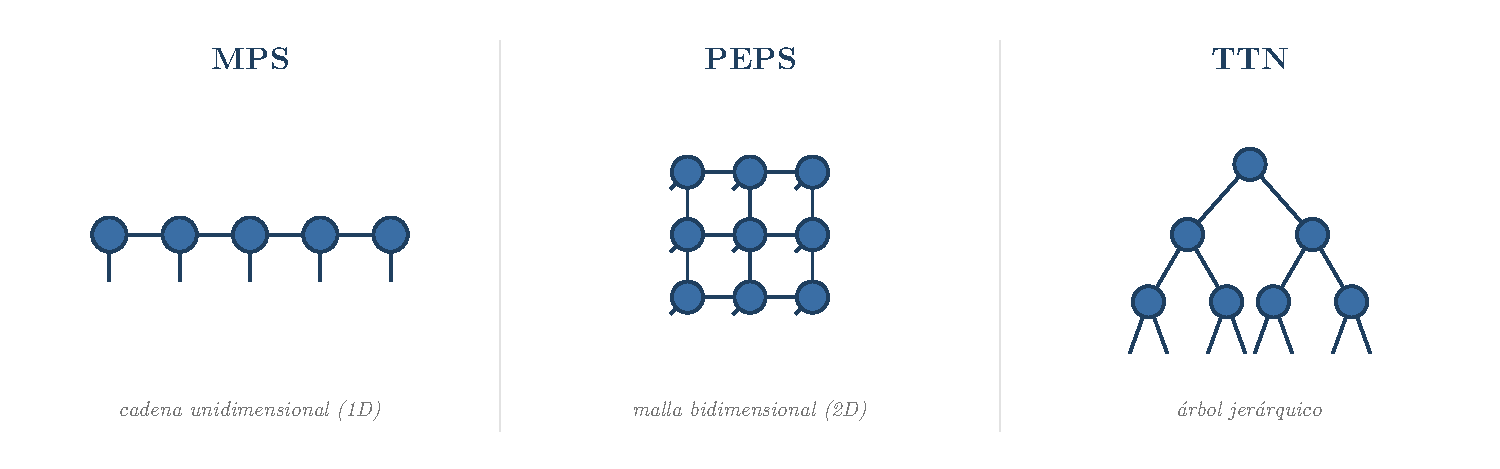
\includegraphics[width=\textwidth]{images/tn_types.pdf}
    \caption{Distintos tipos de redes tensoriales. \textbf{MPS} (\textit{Matrix Product
    State}): cadena unidimensional, la estructura empleada en este trabajo.
    \textbf{PEPS} (\textit{Projected Entangled Pair States}): generalización a una malla
    bidimensional. \textbf{TTN} (\textit{Tree Tensor Network}): red jerárquica en forma
    de árbol. Las líneas abiertas representan índices físicos y las líneas internas,
    índices de enlace.}
    \label{fig:tn_types}
\end{figure}

En concreto, en este trabajo parametrizamos la función de onda utilizando un \textit{Matrix Product State} (MPS) \cite{orus2014practical}, una de las formas más simples y utilizadas de red tensorial. Un MPS descompone el tensor de coeficientes de una función de onda en una cadena unidimensional de $N$ tensores, asociando un tensor a cada una de las $N$ variables del sistema. Cada tensor posee un índice físico $v_k$ (\textit{physical index}) de dimensión $d_k$, que representa los $d_k$ posibles estados de esa variable, junto con uno o dos índices de enlace que lo conectan con sus vecinos en la cadena. En este trabajo, se utiliza un MPS con condiciones de contorno abiertas, por lo que el primer y el último tensor no están conectados entre sí y disponen de un único índice de enlace.

Matemáticamente, una función de onda parametrizada mediante MPS con condiciones de contorno abiertas es:
\begin{equation}
\Psi(v_1, v_2, \ldots, v_N)
=
\sum_{\alpha_1,\ldots,\alpha_{N-1}}
A^{(1)}_{v_1 \alpha_1}
A^{(2)}_{\alpha_1 v_2 \alpha_2}
\cdots
A^{(N)}_{\alpha_{N-1} v_N}.
\label{eq:mps}
\end{equation}
donde cada $A^{(k)}$ es un tensor del MPS asociado a la variable $v_k$. Cada tensor posee un índice físico $v_k$, cuya dimensión $d_k$ se denomina dimensión física, y uno o dos índices de enlace, $\alpha_{k-1}$ y $\alpha_k$, cuyas dimensiones $D_{k-1}$ y $D_k$ se denominan dimensiones de enlace. En condiciones de contorno abiertas, los tensores de los extremos solo tienen un índice de enlace, lo que puede interpretarse equivalentemente tomando $D_0 = D_N = 1$. Para una observación concreta $\mathbf{v}=(v_1,\ldots,v_N)$, el valor de cada característica $v_k$ selecciona una matriz del tensor correspondiente, que será un vector en el caso del primer y el último tensor. La contracción de estas matrices y vectores a lo largo de la cadena nos devuelve el escalar $\Psi(\mathbf{v})$.

\begin{figure}[H]
    \centering
    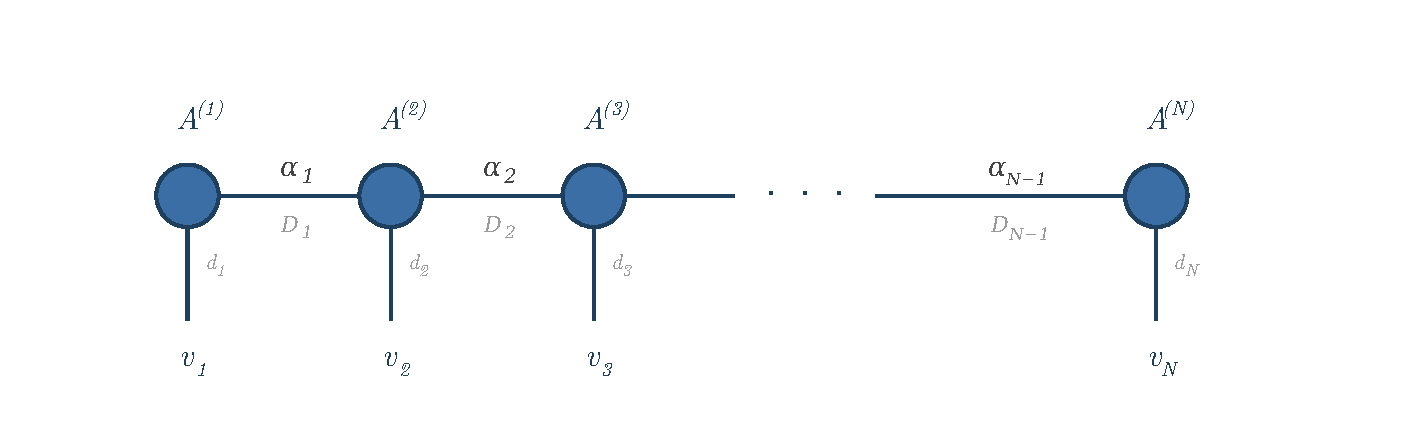
\includegraphics[width=0.85\textwidth]{images/mps_diagram.pdf}
    \caption{Representación gráfica de un \textit{Matrix Product State} (MPS) con
    condiciones de contorno abiertas. Cada tensor $A^{[j]}$ se asocia a una variable
    del sistema y posee un índice físico $s_j$ de dimensión $d$ (líneas verticales) y
    uno o dos índices de enlace $\alpha_k$ de dimensión $\chi$ (líneas horizontales),
    que se contraen a lo largo de la cadena. Los tensores de los extremos cuentan con
    un único índice de enlace.}
    \label{fig:mps}
\end{figure}

Una de las principales ventajas es la eficiencia del MPS para representar la función de onda con un menor número de parámetros necesarios. Mientras que una representación explícita de la función de onda requiere almacenar $\prod_{k=1}^{N} d_k$ coeficientes, un MPS con condiciones de contorno abiertas requiere almacenar
\[
d_1D_1 + \sum_{k=2}^{N-1} D_{k-1}d_kD_k + D_{N-1}d_N
\]
parámetros. Si denotamos por $d_{\max}$ la mayor dimensión física y por $D_{\max}$ la mayor dimensión de enlace, este número queda acotado por $\mathcal{O}(N d_{\max} D_{\max}^2)$. Por tanto, siempre que $d_{\max}$ y $D_{\max}$ se mantengan acotados o crezcan moderadamente con $N$, la representación escala de forma polinómica con el número de variables. Sin embargo, esta reducción de parámetros conlleva un compromiso, puesto que las dimensiones de enlace determinan la cantidad de correlaciones que el MPS puede capturar entre distintas partes del sistema. Valores pequeños de $D_k$ producen representaciones más compactas y computacionalmente eficientes, mientras que valores mayores aumentan la capacidad expresiva de la red a costa de un mayor número de parámetros y un mayor coste de contracción.

Otra ventaja de esta parametrización frente a otros modelos generativos es que la función de partición $Z$ se puede calcular de forma exacta de manera exacta y eficiente. En los modelos basados en energía como las máquinas de Boltzmann \cite{ackley1985boltzmann} la función de partición suele ser intratable y obliga a recurrir a aproximaciones, ya que la suma $\sum_{\mathbf{v} \in \mathcal{V}}$ recorre las $\prod_{k=1}^{N} d_k$ configuraciones posibles, un número que crece exponencialmente con $N$. Sin embargo, la estructura del MPS permite evitar esa suma explícita. Como $\Psi(\mathbf{v})$ es un producto de matrices (\hyperref[eq:mps]{Ecuación~\ref*{eq:mps}}), la norma $Z$ se obtiene
contrayendo el MPS con su conjugado.
\begin{equation}
    Z = \sum_{\mathbf{v}} |\Psi(\mathbf{v})|^2
      = \sum_{\mathbf{v}} \Psi^{*}(\mathbf{v})\,\Psi(\mathbf{v})
      = \langle \Psi | \Psi \rangle .
    \label{eq:Z}
\end{equation}
Gráficamente, esto equivale a colocar una copia conjugada del MPS sobre la red original y conectar entre sí los índices físicos correspondientes, como se observa en la \hyperref[fig:z_contraction]{Figura~\ref*{fig:z_contraction}}. Al contraer cada índice físico $v_k$, se suma localmente sobre los posibles valores de la variable $k$. Como estas sumas se realizan tensor a tensor a lo largo de la cadena, se evita construir o recorrer explícitamente el espacio completo de configuraciones. En la práctica, la contracción se acumula recorriendo la cadena de izquierda a derecha en un entorno parcial $E$, una matriz sobre los índices de enlace que incorpora un nuevo sitio en cada paso. 
\begin{equation}
    E^{(k)}_{\alpha_k,\,\alpha'_k}
    = \sum_{v_k,\;\alpha_{k-1},\;\alpha'_{k-1}}
      \bigl(A^{(k)}_{\alpha'_{k-1}\, v_k\, \alpha'_k}\bigr)^{*}\,
      E^{(k-1)}_{\alpha_{k-1},\,\alpha'_{k-1}}\,
      A^{(k)}_{\alpha_{k-1}\, v_k\, \alpha_k} .
    \label{eq:entorno}
\end{equation}
La clave de la eficiencia es que en ningún momento aparece un tensor de dimensión exponencial, puesto que el entorno $E$ nunca supera el tamaño $D_k \times D_k$. Por ello, si las dimensiones físicas y de enlace permanecen acotadas, el coste de calcular $Z$ escala polinómicamente con $N$, en lugar de exponencialmente.

\begin{figure}[H]
    \centering
    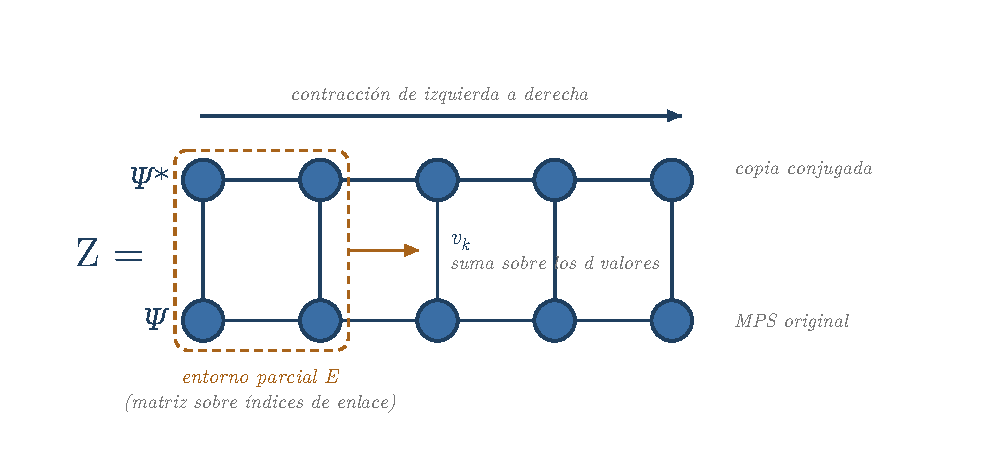
\includegraphics[width=0.9\textwidth]{images/z_contraction.pdf}
    \caption{Cálculo de la función de partición $Z = \langle \Psi | \Psi \rangle$ de un
    MPS. Se coloca una copia conjugada ($\Psi^{*}$) sobre el MPS original ($\Psi$) y se
    conectan los índices físicos correspondientes (líneas verticales); contraer cada uno
    suma localmente sobre los $d$ valores de la variable. La contracción se realiza
    tensor a tensor a lo largo de la cadena, acumulando un entorno parcial $E$ que es una
    matriz sobre los índices de enlace, sin construir nunca un tensor de dimensión
    exponencial. Al no quedar índices abiertos, el resultado es el escalar $Z$.}
    \label{fig:z_contraction}
\end{figure}

\paragraph{Puntuación de anomalía}
\label{par:puntuacionanomalia}
\mbox{}\\

El cálculo exacto de la función de partición $Z$ permite calcular la probabilidad de cada observación de manera exacta mediante la \hyperref[eq:reglaborn]{regla de Born~(\ref*{eq:reglaborn})}:
\begin{equation}
P(\mathbf{v}) = \frac{|\Psi(\mathbf{v})|^2}{Z},
\qquad
Z = \sum_{\mathbf{v}} |\Psi(\mathbf{v})|^2 .
\label{eq:prob}
\end{equation}
El modelo se entrena exclusivamente con observaciones benignas, de modo que el MPS aprende su distribución y asigna probabilidades altas a las observaciones que se ajustan a esa distribución del comportamiento normal y probabilidades bajas a las que se alejan de ella, lo que permite emplear la propia
probabilidad como criterio para la detección de anomalías.

Como puntuación de anomalía, se emplea la verosimilitud logarítmica negativa (\textit{negative log-likelihood}, NLL) \cite{han2018unsupervised}:
\begin{equation}
s(\mathbf{v}) = \mathrm{NLL}(\mathbf{v})
= -\log P(\mathbf{v}).
\label{eq:nll}
\end{equation}
La NLL invierte la escala de la probabilidad, de manera que cuanto menos probable es una observación bajo el modelo, mayor es su puntuación. Además, trabajar en el dominio logarítmico mejora la estabilidad numérica del cálculo, ya que reduce los problemas numéricos derivados de manejar probabilidades extremadamente pequeñas.

Sustituyendo la probabilidad obtenida con la regla de Born, la puntuación de anomalía puede expresarse como:
\begin{equation}
s(\mathbf{v}) = \mathrm{NLL}(\mathbf{v})
= -\log P(\mathbf{v})
= \log Z - \log |\Psi(\mathbf{v})|^2 .
\label{eq:nllcompleta}
\end{equation}
Esta expresión relaciona directamente la puntuación de anomalía con la función de onda aprendida por el MPS. Para un valor fijo de $Z$, una observación con una amplitud $|\Psi(\mathbf{v})|^2$ alta tendrá una NLL baja y, por tanto, será considerada compatible con el comportamiento normal. Por el contrario, una observación con una amplitud baja dará lugar a una NLL elevada, lo que indica que el modelo la considera poco probable y, en consecuencia, potencialmente anómala.

\subsubsection{Codificación de características}
\label{subsubsec:codificacioncaracteristicas}

El modelo MPS opera sobre índices físicos discretos. Cada sitio del MPS está asociado a una característica de la observación y recibe, para dicha característica, un índice entero en el rango $[0, d_k)$, que selecciona una de las $d_k$ componentes del tensor local correspondiente.

Sin embargo, las características de las observaciones son heterogéneas, ya que pueden incluir variables categóricas, binarias y numéricas. Por este motivo, es necesario transformar cada una de ellas en un índice entero compatible con la representación del MPS. Esta etapa es la que da respuesta al requisito de robustez frente a características heterogéneas descrita en \ref{par:requisitosnofuncionales}

\paragraph{Principios de diseño}
\label{par:principiosdiseno}
\mbox{}\\

La codificación se rige por dos principios de diseño que se derivan directamente de los requisitos del sistema.

El primer principio es que el codificador se ajusta exclusivamente sobre las observaciones benignas del conjunto de entrenamiento. Esto significa que todas las decisiones que dependen de los datos, como la construcción de vocabulario de las variables categóricas o la definición de los límites de los intervalos de discretización de las variables numéricas, se toman observando únicamente las observaciones benignas del conjunto de entrenamiento. Este principio responde a la naturaleza semi-supervisada del sistema, puesto que el modelo no debe tener información sobre los ataques ni el conjunto de test.

El segundo principio es el determinismo. Igual que el resto del sistema, el codificador debe asegurar la reproducibilidad y la trazabilidad exigidas por los requisitos. En este caso, dado un mismo conjunto de entrenamiento, el codificador siempre producirá el mismo esquema de codificación y transformará de manera consistente cualquier nueva observación.

\paragraph{Política de asignación de tipo}
\label{par:politicaasignaciontipo}
\mbox{}\\

El codificador no aplica un tratamiento uniforme a todas las características, sino que clasifica cada una en uno de cuatro tipos y le aplica la regla de codificación correspondiente.

En primer lugar, las variables intrínsecamente categóricas se asignan al tipo categórico. Estas variables representan valores simbólicos o etiquetas sin una relación ordinal o métrica necesariamente definida.

Las variables numéricas que siempre toman el mismo valor en el conjunto de entrenamiento se asignan al tipo constante. En esta categoría también se incluyen aquellas que toman el mismo valor en casi todas las observaciones, definiendo "casi todas" como una proporción mayor a un umbral definido en la configuración del codificador.

En tercer lugar, las variables numéricas que toman un número reducido de valores distintos en el conjunto de entrenamiento se asignan al tipo discreto. En este caso, se considera que el número de valores distintos es reducido cuando no supera un umbral definido en la configuración del codificador.

Finalmente, el resto de variables numéricas se asignan al tipo numérico. Estas variables presentan una variabilidad mayor y, por tanto, requieren un proceso específico de discretización antes de poder ser utilizadas como índices físicos del MPS.

\paragraph{Codificación de cada tipo}
\label{par:codificacioncadatipo}
\mbox{}\\

Una vez asignado el tipo de cada característica, la conversión de un valor concreto en un índice entero se realiza según la regla de codificación correspondiente.

Una característica categórica se codifica mediante un vocabulario construido a partir de los valores observados en el conjunto de entrenamiento, que asigna un índice distinto a cada valor observado. La dimensión física resultante es igual al número de valores distintos más uno, ya que se reserva un índice adicional para representar valores no vistos durante el ajuste del codificador.

Una característica constante se codifica de forma binaria con dimensión física dos. El índice 0 indica que el valor es igual al valor característico del conjunto de entrenamiento, y el índice 1 indica que el valor es distinto. De este modo, el modelo recibe directamente la señal de si la característica mantiene el comportamiento observado o se desvía de él.

Una característica discreta se codifica igual que una categórica, siendo su vocabulario los distintos valores presentes en el conjunto de entrenamiento. Al igual que en el caso categórico, se reserva un índice adicional para valores no observados durante el ajuste del codificador.

Finalmente, una característica numérica se codifica discretizando los valores en distintos intervalos, cuyos límites son los cuantiles de la distribución del conjunto de entrenamiento, añadiendo límites infinitos en los intervalos extremos. El uso de cuantiles, en lugar de intervalos de igual anchura, hace que cada intervalo contenga aproximadamente la misma proporción de observaciones benignas. Esto resulta especialmente adecuado para las características con distribuciones de cola larga, en las que una discretización de anchura uniforme dejaría algunos intervalos vacíos o sobrecargados. El índice asignado a cada valor corresponde al intervalo en el que cae dicho valor.

\subsubsection{Algoritmo de entrenamiento DMRG}
\label{subsubsec:algoritmoentrenamiento}

El modelo se entrena por máxima verosimilitud, de forma que los tensores del MPS se ajustan para maximizar la probabilidad que el modelo asigna al conjunto de entrenamiento. Por la monotonía del logaritmo, maximizar la verosimilitud equivale a minimizar la log-verosimilitud negativa (NLL) media sobre dicho conjunto, que se adopta como función de pérdida. Utilizando la definición de la NLL propuesta en la \hyperref[par:puntuacionanomalia]{Sección~\ref*{par:puntuacionanomalia}} y denotando por $B$ un \textit{minibatch} de observaciones normales, se tiene que la función objetivo $\mathcal{L}$ es:

\begin{equation}
    \mathcal{L}
    = \frac{1}{|B|} \sum_{\mathbf{v} \in B} \mathrm{NLL}(\mathbf{v})
    = \frac{1}{|B|} \sum_{\mathbf{v} \in B} \left( \log Z - \log |\Psi(\mathbf{v})|^2 \right)
    = \log Z - \frac{1}{|B|} \sum_{\mathbf{v} \in B} \log |\Psi(\mathbf{v})|^2 .
    \label{eq:funcionperdida}
\end{equation}

En lugar de aplicar descenso de gradiente sobre todos los tensores del MPS a la vez, el entrenamiento emplea un algoritmo de barrido inspirado en el \textit{Density Matrix Renormalization Group} \cite{schollwock2011dmrg}, adaptado al entrenamiento generativo de MPS siguiendo el enfoque de Han~et~al.~\cite{han2018unsupervised}. La idea central es optimizar la cadena por parejas de sitios contiguos, recorriendo la cadena de un extremo a otro de forma repetida. La principal ventaja de este enfoque es que, al separar de nuevo cada pareja de sitios mediante una descomposición en valores singulares, la dimensión de enlace $D_k$ de ese punto de la cadena puede ajustarse de forma adaptativa a la correlación que realmente existe allí, en lugar de fijarse a priori a un valor uniforme para todos los enlaces \cite{han2018unsupervised}. La \hyperref[fig:dmrg]{Figura~\ref*{fig:dmrg} }resume el funcionamiento general del algoritmo de entrenamiento DMRG, cuyos elementos principales se describen a continuación.

\begin{figure}[H]
    \centering
    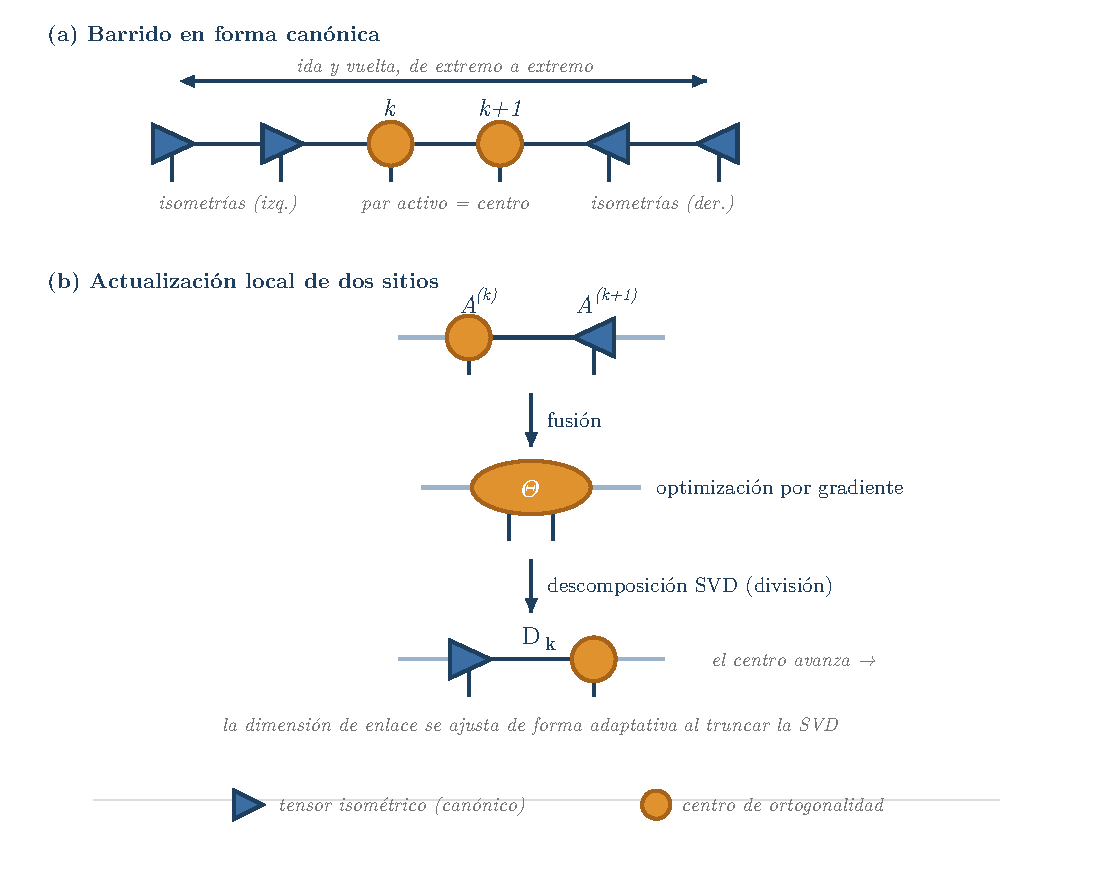
\includegraphics[width=\textwidth]{images/dmrg_sweep.pdf}
    \caption{Esquema del algoritmo de barrido tipo DMRG. (a)~El MPS se mantiene en
    forma canónica: los tensores a ambos lados del par activo son isometrías
    (triángulos orientados hacia el centro) y la optimización recorre la cadena de un
    extremo a otro de forma repetida. (b)~En cada paso local, la pareja de sitios
    activa se fusiona en un único tensor $\Theta$, se optimiza por descenso de
    gradiente y se vuelve a separar mediante una descomposición en valores singulares
    (SVD); el truncamiento de la SVD ajusta de forma adaptativa la dimensión de enlace
    $D_k$ y el centro de ortogonalidad avanza un sitio.}
    \label{fig:dmrg}
\end{figure}

\paragraph{Forma canónica y entornos}
\mbox{}\\

Antes de comenzar el entrenamiento, el estado se normaliza y se lleva a su forma canónica. Esta forma canónica se explica en detalle en el \hyperref[sec:zycanon]{Anexo~\ref*{sec:zycanon}}, y permite que el algoritmo sea más eficiente. En cada actualización local, el centro de ortogonalidad se sitúa sobre la pareja de sitios $(k, k+1)$ que se está optimizando, fusionada en un único tensor de dos sitios $\Theta$.

\begin{equation}
    \Theta_{\alpha_{k-1}\, v_k\, v_{k+1}\, \alpha_{k+1}}
    = \sum_{\alpha_k}
      A^{(k)}_{\alpha_{k-1}\, v_k\, \alpha_k}\,
      A^{(k+1)}_{\alpha_k\, v_{k+1}\, \alpha_{k+1}} .
    \label{eq:merged}
\end{equation}

Como consecuencia, al calcular $Z = \langle \Psi | \Psi \rangle$, los tensores situados a la izquierda y a la derecha del centro se comportan como isometrías y, al contraerse con sus conjugados, colapsan sucesivamente a la identidad. Por tanto, la contracción de toda la cadena se simplifica hasta reducirse a la norma al cuadrado de la pareja de sitios central
\begin{equation}
    Z = \langle \Psi | \Psi \rangle
      = \sum_{\alpha_{k-1},\, v_k,\, v_{k+1},\, \alpha_{k+1}}
        \bigl| \Theta_{\alpha_{k-1}\, v_k\, v_{k+1}\, \alpha_{k+1}} \bigr|^2 ,
    \label{eq:znorm}
\end{equation}
por lo que no es necesario recorrer la cadena completa en cada paso y el algoritmo resulta mucho más eficiente.

Para reducir aún más el coste de cada actualización local se emplean entornos. El entorno izquierdo $L_{\mathbf{v}}$ de un enlace es la contracción de todos los sitios situados a su izquierda para una observación $\mathbf{v}$, y el entorno derecho $R_{\mathbf{v}}$ la de todos los sitios situados a su derecha. 
\begin{align}
    \bigl(L_{\mathbf{v}}\bigr)_{\alpha_{k-1}}
    &= \sum_{\alpha_1,\, \ldots,\, \alpha_{k-2}}
       A^{(1)}_{v_1\, \alpha_1}
       \cdots
       A^{(k-1)}_{\alpha_{k-2}\, v_{k-1}\, \alpha_{k-1}} ,
    \label{eq:envL}\\[2pt]
    \bigl(R_{\mathbf{v}}\bigr)_{\alpha_{k+1}}
    &= \sum_{\alpha_{k+2},\, \ldots,\, \alpha_{N-1}}
       A^{(k+2)}_{\alpha_{k+1}\, v_{k+2}\, \alpha_{k+2}}
       \cdots
       A^{(N)}_{\alpha_{N-1}\, v_N} ,
    \label{eq:envR}
\end{align}
donde los índices físicos quedan fijados a los valores de la observación $\mathbf{v}$.
Con ellos, la amplitud se factoriza a través del centro como
\begin{equation}
    \Psi(\mathbf{v})
    = \sum_{\alpha_{k-1},\, \alpha_{k+1}}
      \bigl(L_{\mathbf{v}}\bigr)_{\alpha_{k-1}}\,
      \Theta_{\alpha_{k-1}\, v_k\, v_{k+1}\, \alpha_{k+1}}\,
      \bigl(R_{\mathbf{v}}\bigr)_{\alpha_{k+1}} .
    \label{eq:psienv}
\end{equation}
Estas contracciones parciales se almacenan en memoria y se actualizan de forma incremental a medida que el centro de ortogonalidad se desplaza durante el barrido. Por ejemplo, al avanzar el centro hacia la derecha, el entorno izquierdo crece incorporando un único sitio,
\begin{equation}
    \bigl(L^{(j)}_{\mathbf{v}}\bigr)_{\alpha_j}
    = \sum_{\alpha_{j-1}}
      \bigl(L^{(j-1)}_{\mathbf{v}}\bigr)_{\alpha_{j-1}}\,
      A^{(j)}_{\alpha_{j-1}\, v_j\, \alpha_j} ,
    \label{eq:envupdate}
\end{equation}
y de forma análoga el entorno derecho al avanzar hacia la izquierda. De este modo, pasar de un enlace al siguiente no requiere volver a contraer la cadena completa, sino únicamente incorporar el sitio correspondiente al entorno adecuado.

\paragraph{Actualización local de dos sitios}
\mbox{}\\

El algoritmo actúa sobre un único enlace $k$, que une los sitios $k$ y $k+1$. En primer lugar, ambos tensores se fusionan en un único tensor $\theta$ de orden cuatro, que conserva los índices de enlace externos y los dos índices físicos. Sobre este tensor fusionado se pueden aplicar uno o varios pasos de descenso de gradiente. Una vez actualizado, $\theta$ se vuelve a separar en dos tensores mediante una descompoosición en valores singulares (SVD). Durante esta descomposición se truncan los valores singulares más pequeños, lo que fija la nueva dimensión de enlace $D_k$. La fracción de norma eliminada en ese truncamiento, que denominamos "peso descartado", cuantifica cuánta información se ha perdido. Además, la SVD traslada el centro de ortogonalidad al siguiente tensor del barrido, de manera que la cadena queda en forma canónica y lista para la siguiente actualización.

\begin{algorithm}[H]
\caption{Actualización local de dos sitios}
\label{alg:actualizacionlocal}
\begin{algorithmic}[1]
\Require Tensores $A^{(k)}$, $A^{(k+1)}$; entornos $L$, $R$; minibatch $B$; tasa de aprendizaje $\eta$; cota $D_{\max}$; tolerancia SVD $\varepsilon$; dirección del barrido
\State $\theta \gets \textsc{Fusionar}(A^{(k)}, A^{(k+1)})$ \Comment{tensor de dos sitios}
\For{$\text{paso} = 1 \text{ a } n_{\text{desc}}$}
    \State $g \gets \nabla_{\theta}\,\mathcal{L}(\theta;\, L, R, B)$ \Comment{Ecuación \ref{eq:gradientenll}}
    \If{$g$ no es finito}
        \State \textbf{continuar} \Comment{se descarta el paso}
    \EndIf
    \State $\theta \gets \theta - \eta\, g$
\EndFor
\State $U, S, V^{\dagger} \gets \textsc{SVD}(\theta)$
\State $(A^{(k)}, A^{(k+1)}),\, w_{\text{desc}} \gets \textsc{Truncar}(U, S, V^{\dagger}, D_{\max}, \varepsilon, \text{dirección})$ \Comment{fija $D_k$}
\State \Return $A^{(k)}$, $A^{(k+1)}$, $w_{\text{desc}}$
\end{algorithmic}
\end{algorithm}

\paragraph{Gradiente de la función de pérdida}
\mbox{}\\

El gradiente de la función objetivo respecto al tensor fusionado $\theta$ admite una forma cerrada \cite{han2018unsupervised}, explicada en el Anexo \ref{sec:zycanon}.

\begin{equation}
\frac{\partial \mathcal{L}}{\partial \theta}
= \frac{2\,\theta}{Z}
- \frac{2}{|B|}\sum_{\mathbf{v}\in B}\frac{L_{\mathbf{v}}\otimes R_{\mathbf{v}}}{\Psi(\mathbf{v})}
\label{eq:gradientenll}
\end{equation}

El primer término, $\frac{2\,\theta}{Z}$ procede de la derivada de $\log{Z}$. Este término actúa como término de normalización, puesto que empuja la amplitud del modelo a la baja de manera global para que la probabilidad total siga sumando uno.

El segundo término es el que incrementa la amplitud en las configuraciones presentes en el minibatch, ponderando cada una por el inverso de su amplitud $\Psi(\mathbf{v)}$, de modo que las observaciones a las que el modelo todavía asigna poca amplitud reciben una corrección mayor.

El equilibrio entre ambos términos es lo que conduce al modelo a concentrar amplitud, y por tanto probabilidad, sobre las regiones que se parecen al tráfico normal, y a retirarla del resto. Conviene notar que el término de normalización es barato de calcular precisamente gracias a la forma canónica, pues en ese punto Z coincide con la norma al cuadrado de $\theta$.

\paragraph{Dimensión de enlace adaptativa}
\mbox{}\\

La cota sobre las dimensiones de enlace introducida en la Sección \ref{par:dimensionenlace} no es estática, sino que comienza en un valor reducido $D_{init}$ y crece de forma multiplicativa a lo largo del entrenamiento hasta el tope máximo $D_{max}$. El crecimiento no es automático en cada loop, sino que está condicionado a que la cota sea limitante. Se considera que la cota es limitante en un loop cuando se da alguna de dos circunstancias: que algún enlace haya alcanzado efectivamente el valor de la cota, lo que indica que la SVD habría querido conservar más rango del permitido, o que el peso descartado en el truncamiento haya superado un umbral prefijado, lo que indica que el truncamiento está eliminando información no despreciable. Solo cuando la cota resulta limitante durante un número de loops consecutivos se aumenta por un factor f.

Este mecanismo tiene una doble justificación. Por un lado, permite que el modelo arranque siendo pequeño y barato y añada capacidad únicamente donde y cuando los datos la reclaman, en coherencia con el requisito de coste computacional acotado, ya que $D_{max}$ acota en todo momento la memoria y el cómputo. Por otro lado, actúa como un mecanismo de regularización, pues la capacidad solo se concede ante evidencia sostenida de que es necesaria, lo que dificulta que el modelo crezca para ajustar ruido en lugar de estructura genuina del tráfico normal.

\paragraph{Control de la convergencia}
\mbox{}\\

El entrenamiento incorpora varios mecanismos con el propósito de que se mantenga estable. En primer lugar, la tasa de aprendizaje se reduce de forma adaptativa cuando la NLL deja de mejorar durante un número de loops igual a la paciencia, multiplicándose por un factor de reducción $rho$ menor que uno. Si la tasa de aprendizaje cae por debajo de un valor mínimo el entrenamiento se detiene. Además, se contempla una parada temprana si la NLL no mejora durante un número prolongado de loops. Finamente, si todos los gradientes de varios loops consecutivos resultan no finitos, situación en la que el entrenamiento no puede progresar, se aborta el entrenamiento. 

A lo largo del proceso se conserva una copia del mejor modelo observado según la métrica de seguimiento, que se restaura al terminar, de modo que el modelo final no es el del último loop sino el mejor de todos.

\paragraph{Barrido y bucle de entrenamiento}
\mbox{}\\

Un barrido consiste en aplicar la actualización local a todos los enlaces de la cadena de forma ordenada. Un barrido a la derecha recorre los enlaces desde $k=0$ hasta $k=N-2$, actualizando en cada paso los tensores $k$ y $k+1$, y desplazando el centro de ortogonalidad hacia la derecha. Un barrido a la izquierda los recorre en sentido inverso. Por cada minibatch se realiza un barrido a la derecha seguido de uno a la izquierda, de manera que todos los enlaces se actualizan dos veces. Un loop de entrenamiento procesa de este modo todos los minibatches. Al final de cada loop el estado se renormaliza y se recanonicaliza, y se mide la NLL sobre el conjunto de entrenamiento y sobre el de validación si está disponible para monitorizar el progreso.

\begin{algorithm}[H]
\caption{Bucle de entrenamiento DMRG}
\label{alg:bucleentrenamiento}
\begin{algorithmic}[1]
\Require Datos de entrenamiento; cota inicial $D_{\text{init}}$; cota máxima $D_{\max}$; tasa de aprendizaje inicial $\eta_0$; número de loops
\State Normalizar y canonicalizar el MPS
\State $D \gets D_{\text{init}}$;\; $\eta \gets \eta_0$;\; $\text{mejor} \gets \infty$
\For{$\text{loop} = 1 \text{ a } n_{\text{loops}}$}
    \ForAll{minibatch $B$}
        \State Construir los entornos $L$, $R$
        \State Barrido a la derecha: Algoritmo \ref{alg:actualizacionlocal} en $k = 0, \ldots, N-2$
        \State Reconstruir los entornos $L$, $R$
        \State Barrido a la izquierda: Algoritmo \ref{alg:actualizacionlocal} en $k = N-2, \ldots, 0$
    \EndFor
    \State Renormalizar y recanonicalizar el MPS
    \State Medir la NLL
    \If{la NLL mejora}
        \State Guardar copia del modelo;\; reiniciar la paciencia
    \Else
        \State Incrementar la paciencia;\; si supera el límite, $\eta \gets \eta \cdot \rho$
    \EndIf
    \If{la cota $D$ ha sido limitante durante varios loops seguidos}
        \State $D \gets \min\!\big(D_{\max},\, \lceil D \cdot f \rceil\big)$
    \EndIf
\EndFor
\State Restaurar la mejor copia del modelo guardada
\end{algorithmic}
\end{algorithm}

\subsubsection{Mecanismo de explicabilidad}
\label{subsubsec:mecanismoexplicabilidad}

\subsection{Implementaci\'on}

\subsubsection{Conjunto de datos utilizado}
\label{subsubsec:conjuntodatos}

\subsubsection{Arquitectura del modelo MPS}
\label{subsubsec:arquitecturamodelo}

\subsubsection{Estructura del código}
\label{subsubsec:estructuracodigo}

\subsubsection{Pipeline}
\label{subsubsec:pipeline}

\subsubsection{Reproducibilidad}
\label{subsubsec:reproducibilidad}

\subsubsection{Tecnologías y recursos empleados}
\label{subsubsec:tecnologiasyrecursos}


\newpage

%%%%%%%%%%%%%%%%%%%%%%%%%%%%%%%%%%%%%%%%%%%%%%%%%%%%%%%%
%%%% Experimentos %%%%%%%%%%%%%%%%%%%%%%%%%%%%%%%%%%%%%%%
%%%%%%%%%%%%%%%%%%%%%%%%%%%%%%%%%%%%%%%%%%%%%%%%%%%%%%%%
\section{Resultados}\label{sec:results}

\subsection{Evaluación}
\label{subsec:evaluacion}

\textcolor{red}{En este capítulo se ha de describir cómo se ha validado la solución y qué resultados se han obtenido según las métricas especificadas en el planteamiento del problema, realizando un análisis crítico de los mismos. También es un capítulo obligatorio y clave, en el que la visualización y la presentación de los resultados serán de suma importancia.
Los resultados obtenidos deberían ser reproducibles, por lo que se deberá aportar toda la información necesaria para ello.
}

\textcolor{blue}{Objetivo de la secci\'on: demostrar cuantitativa y cualitativamente qu\'e tal funcionan los desarrollos realizados}

\newpage

%%%%%%%%%%%%%%%%%%%%%%%%%%%%%%%%%%%%%%%%%%%%%%%%%%%%%%%%
%%%% Conclusiones %%%%%%%%%%%%%%%%%%%%%%%%%%%%%%%%%%%%%%%
%%%%%%%%%%%%%%%%%%%%%%%%%%%%%%%%%%%%%%%%%%%%%%%%%%%%%%%%
\section{Conclusiones y Trabajo Futuro}\label{sec:conclusion}
\textcolor{blue}{Objetivo de la secci\'on: describir en qu\'e medida se han alcanzado los objetivos, en qu\'e otros campos pueden aplicarse los desarrollos, qu\'e mejoras pueden incorporarse al proyecto...}

\newpage

%%%%%%%%%%%%%%%%%%%%%%%%%%%%%%%%%%%%%%%%%%%%%%%%%%%%%%%%
%%%% Referencias %%%%%%%%%%%%%%%%%%%%%%%%%%%%%%%%%%%%%%%
%%%%%%%%%%%%%%%%%%%%%%%%%%%%%%%%%%%%%%%%%%%%%%%%%%%%%%%%
\section{Bibliograf\'ia} \label{sec:bibliography}

\printbibliography[heading=none]

\end{refsection}
\newpage

%%%%%%%%%%%%%%%%%%%%%%%%%%%%%%%%%%%%%%%%%%%%%%%%%%%%%%%%
%%%% Anexos %%%%%%%%%%%%%%%%%%%%%%%%%%%%%%%%%%%%%%%%%%%%
%%%%%%%%%%%%%%%%%%%%%%%%%%%%%%%%%%%%%%%%%%%%%%%%%%%%%%%%
\appendix
\section{Redes Tensoriales y Matrix Product States}
\label{sec:anexoredes}

\end{document}




